% Atualizado para atender as normas ABNT por Mônica da Silva (04/11/2021)

% --- -----------------------------------------------------------------
% --- Elementos usados na Capa e na Folha de Rosto.
% --- EXPRESSÔES ENTRE <> DEVERÂO SER COMPLETADAS COM A INFORMAÇÂO ESPECÍFICA DO TRABALHO
% --- E OS SÌMBOLOS <> DEVEM SER RETIRADOS 
% --- -----------------------------------------------------------------
\autor{MAIQUEL E SILVA GOMES} % deve ser escrito em maiúsculo

\titulo{FRAMEWORK COM INTELIGÊNCIA ARTIFICIAL PARA MODELAGEM SEMÂNTICA DE PROCESSOS DE NEGÓCIO EM BPMN A PARTIR DE LINGUAGEM NATURAL}

\instituicao{UNIVERSIDADE FEDERAL FLUMINENSE}

\orientador{José Viterbo Filho}

\coorientador{Gyslla Vasconcelos} % se nao existir co-orientador apague essa linha

\local{NITERÓI}
%\local{NITER\'{O}I}

\data{2026} % ano da defesa

\comentario{<Tese de Doutorado OU Dissertação de Mestrado> apresentada ao Programa de P\'{o}s-Gradua\c{c}\~{a}o em Computa\c{c}\~{a}o da \mbox{Universidade} Federal Fluminense como requisito parcial para a obten\c{c}\~{a}o do Grau de \mbox{<Doutor ou Mestre> em Computa\c{c}\~{a}o}. \'{A}rea de concentra\c{c}\~{a}o: \mbox{<\'AREA DE CONCENTRA\c{C}\~AO.>}} %preencha com a sua área de concentração


% --- -----------------------------------------------------------------
% --- Capa. (Capa externa, aquela com as letrinhas douradas)(Obrigatório)
% --- ----------------------------------------------------------------
\capa

% --- -----------------------------------------------------------------
% --- Folha de rosto. (Obrigatório)
% --- ----------------------------------------------------------------
\folhaderosto

% --- -----------------------------------------------------------------
% --- Ficha catalográfica obrigatória na versão final. (Obrigatório)
% --- ----------------------------------------------------------------

\begin{figure}[!ht]
   \centering
   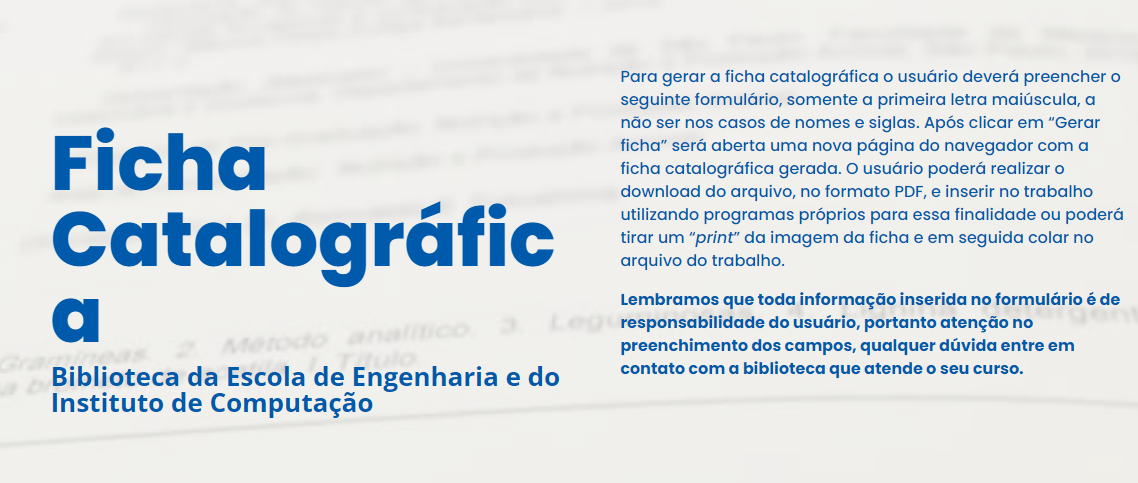
\includegraphics[width=1\linewidth]{capitulos/figuras/ficha_catalografica.png}
   \caption{Local da ficha catalográfica}
\end{figure}

\cleardoublepage


\pagestyle{ruledheader}
\setcounter{page}{1}
\pagenumbering{roman}

% --- -----------------------------------------------------------------
% --- Termo de aprovação. (Obrigatório)
% --- ----------------------------------------------------------------
\cleardoublepage
\thispagestyle{empty}

\vspace{-60mm}

\begin{center}
   {\large <NOME DO ALUNO>}\\
   \vspace{7mm}

   <T\'ITULO DO TRABALHO>\\
  \vspace{10mm}
\end{center}

\noindent
\begin{flushright}
\begin{minipage}[t]{8cm}

<Tese de Doutorado ou Dissertação de Mestrado> apresentada ao Programa de P\'{o}s-Gradua\c{c}\~{a}o em Computa\c{c}\~{a}o da Universidade Federal Fluminense como requisito parcial para a obten\c{c}\~{a}o do \mbox{Grau} de <Doutor ou Mestre> em Computa\c{c}\~{a}o. \'{A}rea de concentra\c{c}\~{a}o: \mbox{<\'AREA DE CONCENTRA\c{C}\~AO.>} %preencha com a sua área de concentração

\end{minipage}
\end{flushright}
\vspace{1.0 cm}
\noindent
Aprovada em <MES> de <ANO>. \\
\begin{flushright}
 % \parbox{11cm}
  {
  \begin{center}
  BANCA EXAMINADORA \\
  \vspace{6mm}
  \rule{11cm}{.1mm} \\
    Prof. <NOME do ORIENTADOR> - Orientador, UFF \\
    \vspace{6mm}
  \rule{11cm}{.1mm} \\
    Prof. <NOME DO AVALIADOR>, <INSTITUI\c{C}\~AO>\\
    \vspace{6mm}
  \rule{11cm}{.1mm} \\
    Prof. <NOME DO AVALIADOR>, <INSTITUI\c{C}\~AO>\\
  \vspace{4mm}
  \rule{11cm}{.1mm} \\
    Prof. <NOME DO AVALIADOR>, <INSTITUI\c{C}\~AO>\\
    \vspace{6mm}
  \rule{11cm}{.1mm} \\
    Prof. <NOME DO AVALIADOR>, <INSTITUI\c{C}\~AO>\\
  \vspace{6mm}
  \end{center}
  }
\end{flushright}
\begin{center}
  \vspace{4mm}
  Niter\'{o}i \\
  %\vspace{6mm}
  <ANO>

\end{center}

% --- -----------------------------------------------------------------
% --- Dedicatoria.(Opcional)
% --- -----------------------------------------------------------------
\cleardoublepage
\thispagestyle{empty}
\vspace*{200mm}

\begin{flushright}
{\em 
  Aos meus pais, pelo amor incondicional e pela crença inabalável
  em cada passo desta jornada.\\[0.5cm]
  À minha orientadora e ao meu orientador,
  pela generosidade intelectual e pela confiança depositada.\\[0.5cm]
  \textit{``A lógica levará você de A a B.
  A imaginação levará você a qualquer lugar.''} --- Albert Einstein
}
\end{flushright}
\newpage


% --- -----------------------------------------------------------------
% --- Agradecimentos.(Opcional)
% --- -----------------------------------------------------------------
\pretextualchapter{Agradecimentos}
\hspace{5mm}
<Elemento opcional, colocado após a dedicatória (ABNT, 2005). >
Ao Prof.\ José Viterbo Filho, orientador desta dissertação, pela
  orientação precisa, pelas discussões que ampliaram meu horizonte de
  pesquisa e pelo incentivo constante à rigorosidade científica.
 
  À Prof.ª Gyslla Vasconcelos, coorientadora, pela dedicação e pelas
  contribuições fundamentais nas etapas de revisão sistemática e de
  análise empírica, especialmente na publicação conjunta no WCIST 2025.
 
  Ao Programa de Pós-Graduação em Computação (PPGC) da Universidade
  Federal Fluminense (UFF) e ao Instituto de Computação (IC-UFF),
  pela infraestrutura, pelo apoio acadêmico e pela formação de
  excelência que tornaram este trabalho possível.
 
  Aos membros da banca examinadora, pela disposição em avaliar este
  trabalho e pelas contribuições que certamente o enriquecerão.
 
  Aos colegas de laboratório e de programa, pelas trocas de ideias,
  pelos momentos de colaboração e pela amizade cultivada ao longo
  deste percurso.
 
  À minha família, pelo suporte emocional e pela compreensão nos
  momentos de ausência que a pesquisa inevitavelmente impõe.
 
  A todos que, direta ou indiretamente, contribuíram para a realização
  deste trabalho, o meu sincero reconhecimento.



% --- -----------------------------------------------------------------
% --- Resumo em português.(Obrigatório)
% --- -----------------------------------------------------------------
\begin{resumo}

A Gestão de Processos de Negócio (BPM) demanda modelos formalizados
  para análise e otimização organizacional, sendo o \textit{Business
  Process Model and Notation} (BPMN) o padrão predominante na indústria.
  Contudo, a construção manual de modelos BPMN é intensiva em mão de
  obra especializada, propensa a inconsistências e representa um
  gargalo significativo nos ciclos de vida BPM. A emergência dos
  Grandes Modelos de Linguagem (LLMs) — como GPT-4, LLaMA e Gemini
  --- abre perspectivas para a transformação automatizada de texto
  em modelo (\textit{text-to-model}). No entanto, evidências empíricas
  apontam para limitações estruturais relevantes: abordagens baseadas
  exclusivamente em LLMs demonstram incapacidade fundamental para
  raciocínio grafo-teórico e otimização espacial exigidos por layouts
  BPMN válidos. Esta dissertação propõe um \textit{framework} híbrido
  que integra extração semântica via LLMs com algoritmos determinísticos
  especializados para geração de layout gráfico, visando superar as
  deficiências identificadas na literatura. Para tanto, realizou-se
  uma revisão rápida de 11 estudos empíricos publicados entre 2023 e
  2025, revelando que 55\% das abordagens falham em processos com
  complexidade não trivial e que 64\% carecem de artefatos reproduzíveis.
  O \textit{framework} proposto adota uma arquitetura em camadas que
  separa responsabilidades semânticas e geométricas, permitindo
  modelagem BPMN a partir de descrições em linguagem natural com
  suporte a estruturas hierárquicas, gateways paralelos e
  colaborações multi-participante. Os resultados preliminares
  demonstram viabilidade da abordagem para processos de Nível 2
  e Nível 3 de complexidade, contribuindo para a maturidade de
  uma área de pesquisa em formação.

{\hspace{-8mm} \bf{Palavras-chave}}: Modelagem de Processos de Negócio.
  BPMN. Grandes Modelos de Linguagem. Geração Automática de Diagramas.
  Processamento de Linguagem Natural. Framework Híbrido.

\end{resumo}

% --- -----------------------------------------------------------------
% --- Resumo em língua estrangeira.(Obrigatório)
% --- -----------------------------------------------------------------
\begin{abstract}

Elemento obrigatório, em língua estrangeira, com as mesmas características do resumo em língua vernácula (ABNT, 2005).


O resumo deve ser redigido na terceira pessoa do singular, com verbo na voz ativa, não ultrapassando uma página ou 500 palavras, segundo a ABNT NBR 6028). Evitando-se ouso de parágrafos no meio do resumo, assim como fórmulas, equações e símbolos. Iniciar o resumo situando o trabalho no contexto geral, apresentar os objetivos, descrever a metodologia utilizada, relatar a contribuição própria, comentar os resultados obtidos e finalmente apresentaras conclusões mais importantes do trabalho.



{\hspace{-8mm} \bf{Keywords}}: Palavras representativas do conteúdo do trabalho, isto é, palavras-chave e/ou descritores, na língua (ABNT, 2005).

\end{abstract}

% --- -----------------------------------------------------------------
% --- Lista de figuras.(Opcional)
% --- -----------------------------------------------------------------
%\cleardoublepage
\listoffigures



% --- -----------------------------------------------------------------
% --- Lista de tabelas.(Opcional)
% --- -----------------------------------------------------------------
\cleardoublepage
%\label{pag:last_page_introduction}
\listoftables
\cleardoublepage

% --- -----------------------------------------------------------------
% --- Lista de abreviatura.(Opcional)
%Elemento opcional, que consiste na relação alfabética das abreviaturas e siglas utilizadas no texto, seguidas das %palavras ou expressões correspondentes grafadas por extenso. Recomenda-se a elaboração de lista própria para cada %tipo (ABNT, 2005).
% --- ----------------------------------------------------------------

\cleardoublepage
\printglossary[type=\acronymtype,title={Lista de Abreviaturas e Siglas}]
\cleardoublepage


% --- -----------------------------------------------------------------
% --- Sumario.(Obrigatório)
% --- -----------------------------------------------------------------

\pagestyle{ruledheader}
\tableofcontents
\pagebreak